\subsection*{Problema 32}

\textbf{Enunciado:} Calcular la integral:
\begin{align*}
\int \dfrac{x^4 - 2x^2 + 3x + 4}{(x - 1)^3 (x^2 + 2x + 2)} \, dx
\end{align*}

\textbf{Solución:} 
El integrando es una función racional propia. 
Utilizamos el método de fracciones parciales 
con factores lineales repetidos y cuadráticos 
irreducibles:
\begin{align*}
\dfrac{x^4 - 2x^2 + 3x + 4}{(x - 1)^3 (x^2 + 2x + 2)} = 
&\dfrac{A}{x - 1} + \dfrac{B}{(x - 1)^2} \\
&+ \dfrac{C}{(x - 1)^3} + \dfrac{Dx + E}{x^2 + 2x + 2}
\end{align*}

Multiplicando ambos lados por el denominador común:
\begin{align*}
x^4 - 2x^2 + 3x + 4 = 
&A(x - 1)^2(x^2 + 2x + 2) \\
&+ B(x - 1)(x^2 + 2x + 2) \\
&+ C(x^2 + 2x + 2) \\
&+ (Dx + E)(x - 1)^3
\end{align*}

Evaluando en $x = 1$:
\begin{align*}
1^4 - 2(1)^2 + 3(1) + 4 &= C(1^2 + 2(1) + 2) \\
6 &= 5C \implies C = \dfrac{6}{5}
\end{align*}

Desarrollando y agrupando coeficientes por potencias de $x$, 
o aplicando derivadas sucesivas para $A$, $B$, $D$ y $E$:
\begin{align*}
A &= -\dfrac{1}{25}, \quad B = \dfrac{17}{5}, \quad C = \dfrac{6}{5}, \\
D &= \dfrac{26}{25}, \quad E = -\dfrac{38}{25}
\end{align*}

Sustituyendo las fracciones parciales e integrando 
término a término:
\begin{align*}
\int &\left( \dfrac{-1/25}{x - 1} + \dfrac{17/5}{(x - 1)^2} + \dfrac{6/5}{(x - 1)^3} \right) dx \\
&+ \int \dfrac{\frac{26}{25}x - \frac{38}{25}}{x^2 + 2x + 2} \, dx
\end{align*}

Resolviendo las tres primeras integrales directas:
\begin{align*}
-\dfrac{1}{25}\ln|x - 1| - \dfrac{17}{5(x - 1)} - \dfrac{3}{5(x - 1)^2}
\end{align*}

Para la integral restante, completamos el trinomio 
en el denominador $x^2 + 2x + 2 = (x + 1)^2 + 1$ 
y ajustamos el numerador:
\begin{align*}
\int \dfrac{\frac{26}{25}x - \frac{38}{25}}{(x + 1)^2 + 1} \, dx = 
\dfrac{13}{25}\ln(x^2 + 2x + 2) \\
- \dfrac{51}{25}\arctan(x + 1)
\end{align*}

Finalmente, unimos todos los resultados y 
agregamos la constante de integración $C_{int}$:
\begin{align*}
F(x) &= -\dfrac{1}{25}\ln|x - 1| + \dfrac{13}{25}\ln(x^2 + 2x + 2) \\
&\quad - \dfrac{17}{5(x - 1)} - \dfrac{3}{5(x - 1)^2} \\
&\quad - \dfrac{51}{25}\arctan(x + 1) + C_{int}
\end{align*}

\begin{figure}[H]
	\centering
	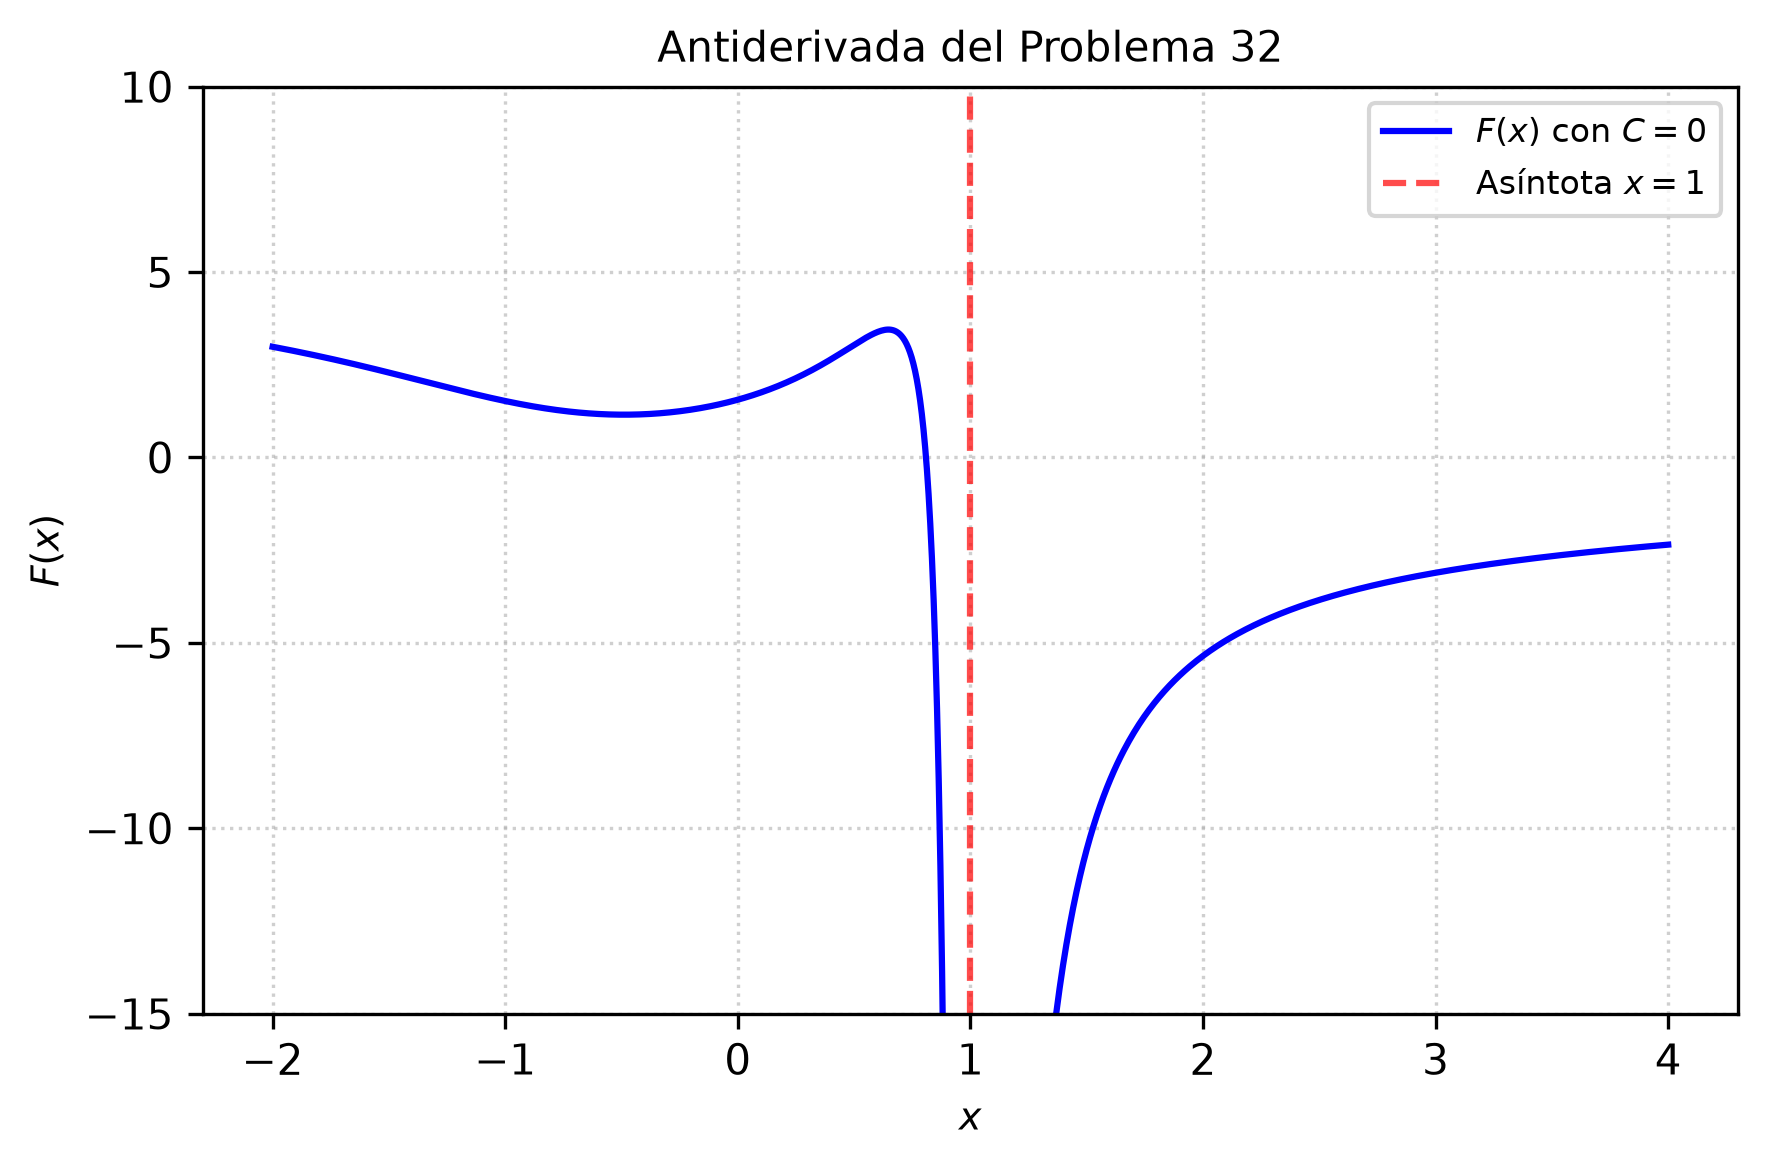
\includegraphics[width=\columnwidth]{semana_03/graficas/SEM03_P32_grafica.png}
	\caption{Representación gráfica de $f(x)$ y su antiderivada $F(x)$ evaluada para la constante de integración $C = 0$ (Problema 32).}
	\label{fig:problema32}
\end{figure}
